\section{Mixnet}

A mixnet (mix network) is a routing protocol designed to provide strong anonymity and resist eavesdropping, even against global adversaries capable of observing the entire network. 
It achieves this by relaying messages through a series of intermediary nodes, called mixnodes, which apply cryptographic transformations to the messages before forwarding them.


Messages are recursively encrypted, creating multiple layers that are peeled off by each mixnode along the path. 
This ensures that each node only knows its immediate predecessor and successor, preventing any single node from accessing both the sender's and the receiver's information. 
Additionally, each encryption layer includes an integrity tag, which prevents tampering and improves the network’s resistance against malicious mixnodes and active adversaries.

Although mixnet shares similarities with onion routing, they differ in key aspects as illustrated by Figure \ref{fig:mixnet_traffic}.
First, mixnet is packet-based, whereas onion routing is circuit-based. 
This means that each packet follows a different path rather than using the same intermediate nodes during the whole communication.
Furthermore, mixnet includes message batching and reordering mechanism to mitigate timing analysis attacks. 
To further prevent correlation, mixnet relies on fixed-size packet format such as Sphinx packet (section \ref{sec:sphinx}), making it difficult for external observers to link incoming and outgoing messages at any given node.

In summary, mixnets provide stronger privacy guarantees than onion routing at the cost of increased latency.

\begin{figure}[h]
    \centering
    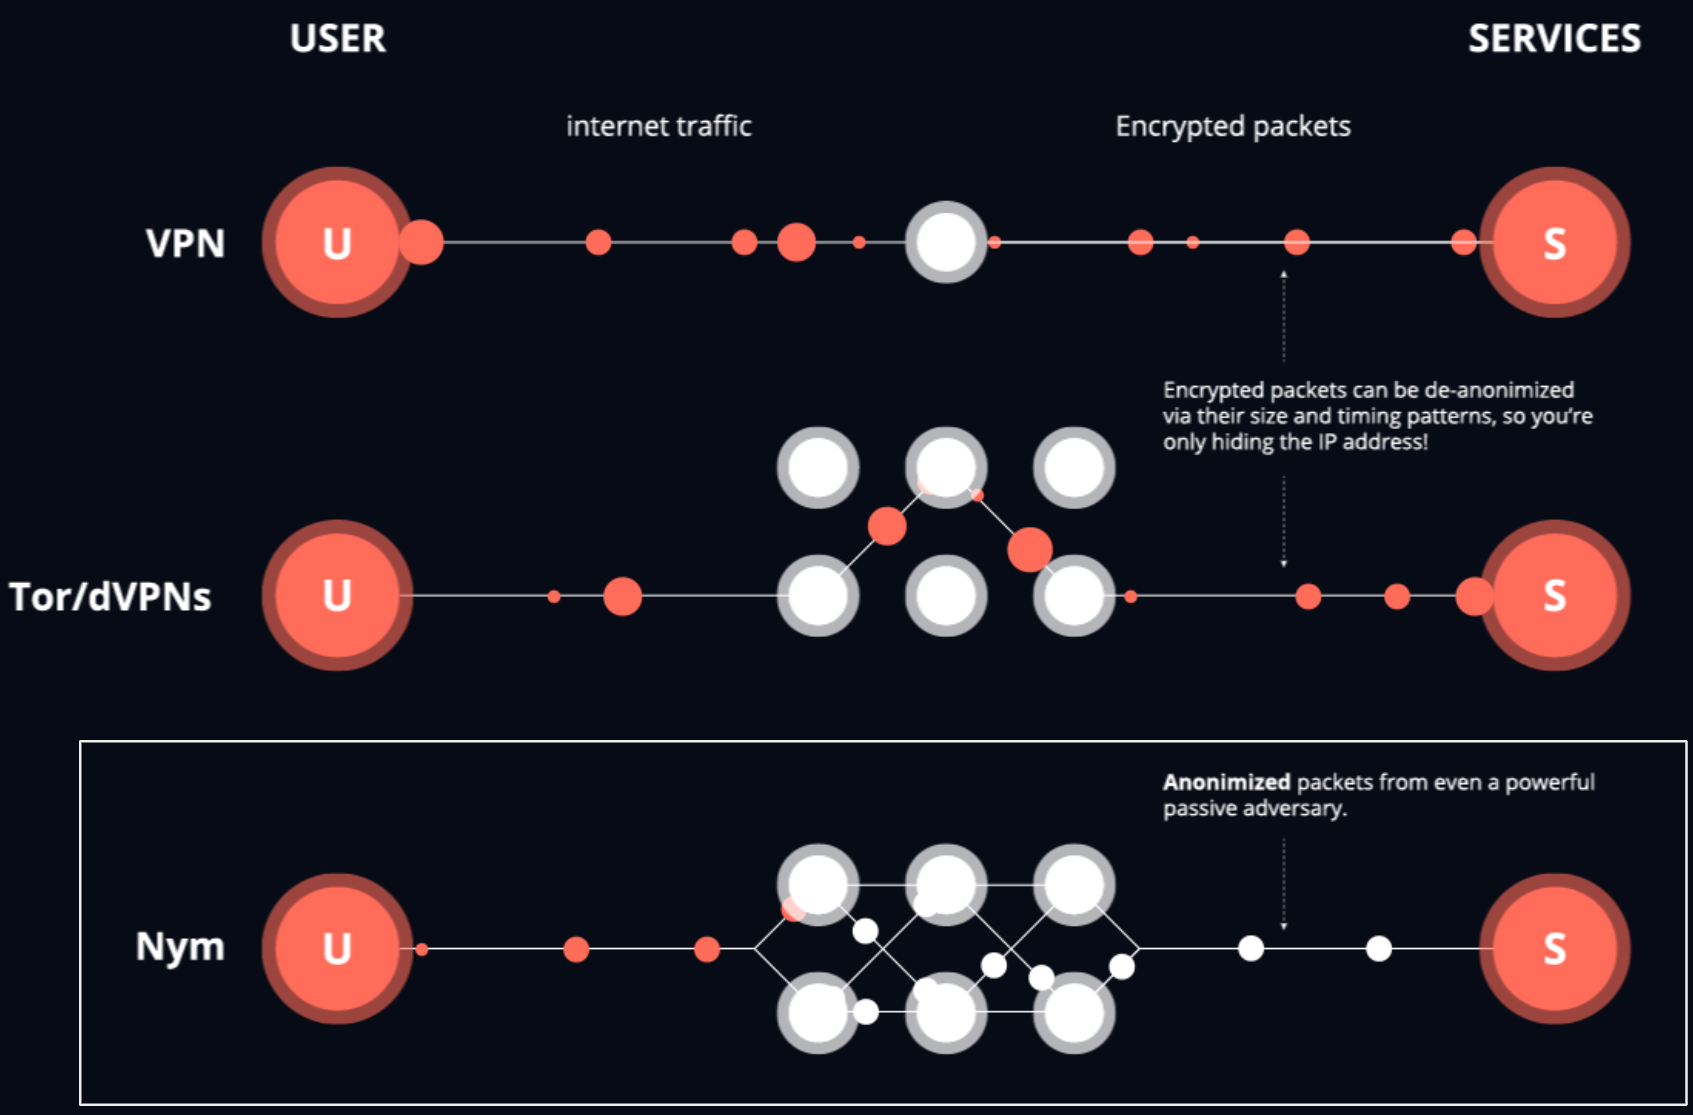
\includegraphics[width=\linewidth]{Images/mixnet_traffic.png}
    \caption{Mixnet traffic compared to TOR and VPN. [source ?]}
    \label{fig:mixnet_traffic}
\end{figure}